%!xelatex = 'xelatex --halt-on-error %O %S'
\documentclass{thuemp}
\begin{document}
\emptitle{OS代码阅读报告}
\empauthor{江灿}{2019011325}
\fancyhead[CO]{{\footnotesize 江灿: Os代码阅读报告}}
\Keyword{光栅衍射,波长,光栅常数,最小偏向角}
\twocolumn[
\begin{@twocolumnfalse}
\maketitle
\begin{empAbstract}
	本次实验是
\end{empAbstract}
% \empfirstfoot{2022-04-03}{软件02}{双日下M}{7号}
\end{@twocolumnfalse}
]
%%%%%%%%%%%%%%%%%%%%%%%%%%%%%%%%%%%%%%%%%%%%%%%%%%%%%%%%%%%%%%%%
%%%%%%%%%%%%%%%%%%%%%%%%%%%%%%%%%%%%%%%%%%%%%%%%%%%%%%%%%%%%%%%%
%%%%%%%%%%%%%%%%%%%%%%%%%%%%%%%%%%%%%%%%%%%%%%%%%%%%%%%%%%%%%%%%
%  正文由此开始
\wuhao 
代码报告基本要求
\begin{itemize}
  \item 重要函数或语句的代码分析与注释
  \item 基本流程分析
  \item 实现概述
  \item 阅后心得
  \item 评分:知识的理解程度,主要技术分析程度,认真程度
\end{itemize}
\part*{Chapter 1 Operatings system interfaces}
\section*{preface}
The job of an operating system is to share a computer among multiple programs and to provide a more useful set of services than the hardware alone supports.And provides services to user programs through an interface\\
\subsection*{What is a good interface :} provides services to user programs through an interface;offer many powerful features to applications\\
\section*{some words}
\begin{itemize}
  \item xv6:mimicking Unix's internal design,the Os
  \item RISV - v : microprocessor (微处理器)
  \item QEMU : mechine simulator(under linux)
  \item knrnel:a special program that provides services to running programs
  \item program(called a process):has memory containing instructions, data, and a stack
  \item instructions:implement the program’s computation
  \item data:variables on which the computation acts
  \item stack:organizes the program’s procedure calls
  \item grep (global search regular expression(RE) and print out the line
  \item cat(concatenate)
\end{itemize}

\begin{figure}[H]
	\centering
	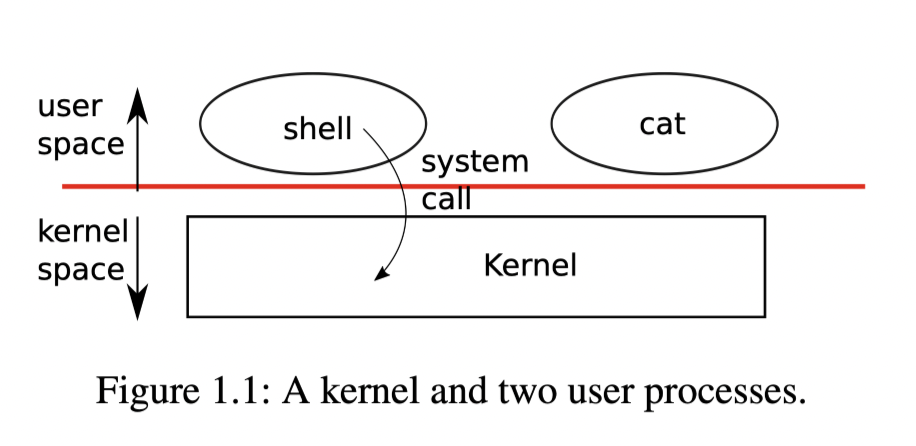
\includegraphics[width=0.8\linewidth]{./image/1.1.png}
	\caption{A kernel and two user processes} 
	\label{png:1.1}
\end{figure}
shell:an ordinary program that reads commands 
from the user and executes them.
The fact that the shell is a user program, 
and not part of the kernel
\newpage
\section*{Processes and memory}
\begin{figure}[H]
	\centering
	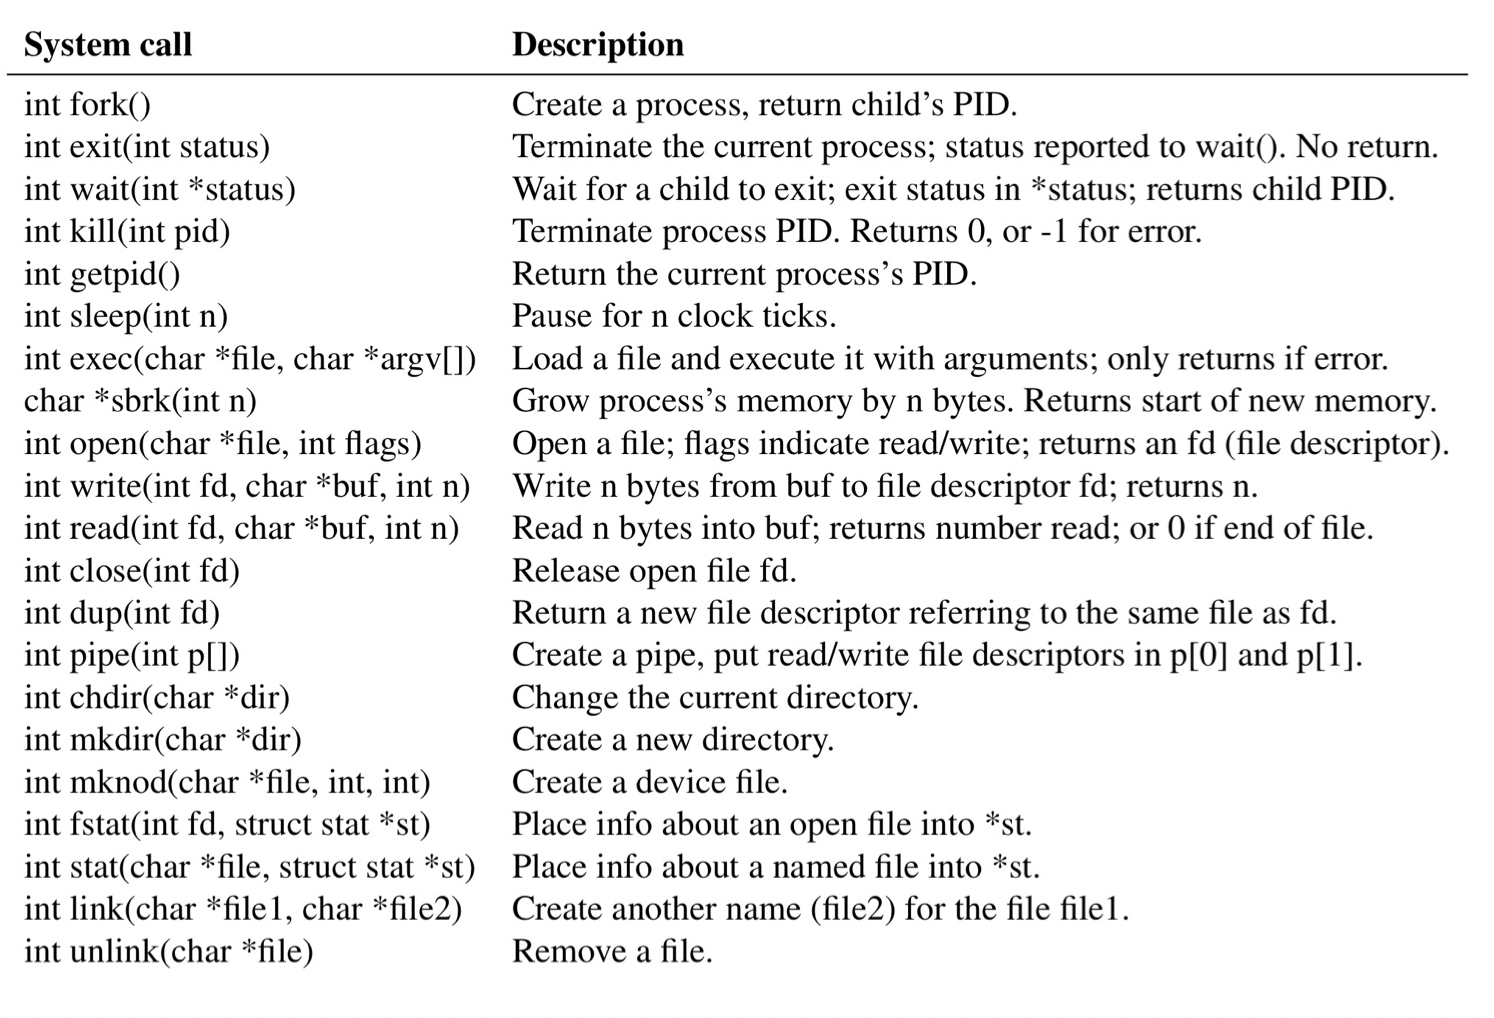
\includegraphics[width=0.8\linewidth]{./image/1.2.png}
	\caption{Xv6 system calls 0(no error)/-1(error)} 
	\label{png:1.2}
\end{figure}
\textbf{PID:} process identifier
$$\mathcal{int \ fork()}$$
system call / give the new process exactly the same memory contents (both instructions and data) as the calling process\\
return original process(new process's PID);\\
new process(0)\\
The physical addresses in parent and child must be different. But C program accesses virtual addresses (if running on an OS that uses virtual memory). The child process gets an exact copy of parent process and virtual address don't change in child process. 
\begin{lstlisting}
      int pid = fork();
  if(pid > 0){
    printf("parent: child = %d\n",pid);
    pid = wait((int *) 0);
    printf("child %d is done\n",pid);
  }else if(pid == 0){
      printf("child : exiting \n");
      exit(0);
  }
  else{
      printf("fork error\n");
  }
\end{lstlisting}
$$\mathcal{int\ exit(int\ status)}$$
0:success
1:failure 
$$\mathcal{int \ wait(int \ *status)}$$
returns the PID of an exited 
(or killed) child of the current process\\ 
copies the exit status of the child to the 
address passed to wait 
no child:-1
pass 1 0 address : don't care about the exit status of a child
$$\mathcal{int \ exec(char \ *file,\ char \ *argv[])}$$
replaces the calling program with an instance of the program\\
argv[0] conventionally the name of the program
$$\mathcal{main}$$
\begin{lstlisting}
  144 int
  145	main(void)
  146	{
  147	  static char buf[100];
  148	  int fd;
  149	
  150	  // Ensure that three file descriptors are open.
  151	  while((fd = open("console", O_RDWR)) >= 0){
  152	    if(fd >= 3){
  153	      close(fd);
  154	      break;
  155	    }
  156	  }
  157	
  158	  // Read and run input commands.
  159	  while(getcmd(buf, sizeof(buf)) >= 0){
  160	    if(buf[0] == 'c' && buf[1] == 'd' && buf[2] == ' '){
  161	      // Chdir must be called by the parent, not the child.
  162	      buf[strlen(buf)-1] = 0;  // chop \n
  163	      if(chdir(buf+3) < 0)
  164	        fprintf(2, "cannot cd %s\n", buf+3);
  165	      continue;
  166	    }
  167	    if(fork1() == 0)//在child 运行
  168	      runcmd(parsecmd(buf));
  169	    wait(0);
  170	  }
  171	  exit(0);
  172	}
\end{lstlisting}
\begin{lstlisting}
8	runcmd(struct cmd *cmd)// while parent run runcmd
78	    exec(ecmd->argv[0], ecmd->argv);//child run exec

\end{lstlisting}
A process that needs more memory at run-time
 (perhaps for malloc) can call sbrk(n) 
 to grow its data memory by n bytes; 
 sbrk returns the location of the new memory.
 \section*{I/O and File descriptors}

 \begin{lstlisting}
  150	  // Ensure that three file descriptors are open.
  151	  while((fd = open("console", O_RDWR)) >= 0){
  152	    if(fd >= 3){//if is 3, break
  153	      close(fd);
  154	      break;
  155	    }
  156	  }
 \end{lstlisting}
%  分栏开始
















\newpage
% \begin{figure}[H]
% 	\centering
% 	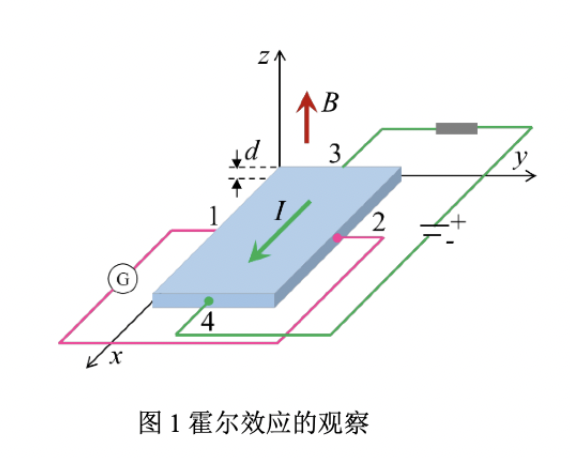
\includegraphics[width=0.8\linewidth]{./image/1.png}
% 	\caption{测定光栅常数和光波波长数据} 
% 	\label{png:1}
% \end{figure}

\begin{lstlisting}
  % 代码段
  \end{lstlisting}






%%%%%%%%%%%%%%%%%%%%%%%%%%%%%%%%%%%%%%%%%%%%%%%%%%
%  参考文献
%%%%%%%%%%%%%%%%%%%%%%%%%%%%%%%%%%%%%%%%%%%%%%%%%%%%%%%%%%%%%%%%
%  参考文献按GB/T 7714-2015《文后参考文献著录规则》的要求著录. 
%  参考文献在正文中的引用方法:\cite{bib文件条目的第一行}

\renewcommand\refname{\heiti\wuhao\centerline{参考文献}\global\def\refname{参考文献}}
\vskip 12pt

\let\OLDthebibliography\thebibliography
\renewcommand\thebibliography[1]{
  \OLDthebibliography{#1}
  \setlength{\parskip}{0pt}
  \setlength{\itemsep}{0pt plus 0.3ex}
}

{
\renewcommand{\baselinestretch}{0.9}
\liuhao
\bibliographystyle{gbt7714-numerical}
\bibliography{./TempExample}
}


\end{document}
